\documentclass{article}
\setlength{\oddsidemargin}{0.25 in}
\setlength{\evensidemargin}{-0.25 in}
\setlength{\topmargin}{-0.6 in}
\setlength{\textwidth}{6.5 in}
\setlength{\textheight}{8.5 in}
\setlength{\headsep}{0.75 in}
\setlength{\parindent}{0 in}
\setlength{\parskip}{0.1 in}

% ===== PACKAGES =====
\usepackage{amsmath,amssymb}
\usepackage{color}
\usepackage{subfigure}
\usepackage{mdframed}
\usepackage{changepage}
\usepackage{graphicx}
\usepackage{url}
\usepackage{enumitem}
\usepackage{multirow}
\usepackage[colorlinks,
            linkcolor=black,
            anchorcolor=blue, 
            citecolor=blue,        
            ]{hyperref}
            
\usepackage{hyperref}
\makeatletter
\def\UrlAlphabet{%
      \do\a\do\b\do\c\do\d\do\e\do\f\do\g\do\h\do\i\do\j%
      \do\k\do\l\do\m\do\n\do\o\do\p\do\q\do\r\do\s\do\t%
      \do\u\do\v\do\w\do\x\do\y\do\z\do\A\do\B\do\C\do\D%
      \do\E\do\F\do\G\do\H\do\I\do\J\do\K\do\L\do\M\do\N%
      \do\O\do\P\do\Q\do\R\do\S\do\T\do\U\do\V\do\W\do\X%
      \do\Y\do\Z}
\def\UrlDigits{\do\1\do\2\do\3\do\4\do\5\do\6\do\7\do\8\do\9\do\0}
\g@addto@macro{\UrlBreaks}{\UrlOrds}
\g@addto@macro{\UrlBreaks}{\UrlAlphabet}
\g@addto@macro{\UrlBreaks}{\UrlDigits}
\makeatother

\newmdenv[
  topline=false,
  bottomline=false,
  skipabove=\topsep,
  skipbelow=\topsep
]{siderules}
\renewcommand{\abstractname}{}

% ===== VARIABLES =====
\def \R{\mathbb{R}}
\def \Pr{\mathbb{P}}
\def \D{{\rm D}}
\def \N{{\rm N}}
\def \xx{{\boldsymbol{\rm x}}}
\def \y{{\rm y}}




% ===== HEADER BOX =====
\newcommand{\lecture}[2]{
\pagestyle{myheadings}
\thispagestyle{plain}
\newpage
\noindent
\begin{center}
\rule{\textwidth}{1.6pt}\vspace*{-\baselineskip}\vspace*{2pt} % Thick horizontal line
\rule{\textwidth}{0.4pt}\\[1\baselineskip] % Thin horizontal line
\vbox{\vspace{2mm}
\hbox to 6.28in { {\bf CS 760: Machine Learning} \hfill Fall 2020 }
\vspace{4mm}
\hbox to 6.28in { {\Large \hfill #1  \hfill} }
\vspace{4mm}
\hbox to 6.28in { {\scshape Authors:}  #2 \hfill }}
\vspace{-2mm}
\rule{\textwidth}{0.4pt}\vspace*{-\baselineskip}\vspace{3.2pt} % Thin horizontal line
\rule{\textwidth}{1.6pt}\\[\baselineskip] % Thick horizontal line
\end{center}
\vspace*{4mm}
}



% =============== DOCUMENT ===============
% \documentclass{book}
\usepackage{graphicx} % [demo]

\usepackage[toc,page]{appendix} % 
\begin{document}

\renewcommand{\baselinestretch}{0.75}\normalsize
\tableofcontents
\renewcommand{\baselinestretch}{1.0}\normalsize

\newcommand{\hytt}[1]{\texttt{\hyphenchar\font=\defaulthyphenchar #1}}


\lecture{Predicting if a Business in America will Survive COVID-19}{Mu Cai(mcai44), Varun Sreenivasan(vsreenivasan), Niharika Tomar(ntomar){@wisc.edu}}


\begin{center}
{\Large {\sf GO GREEN. AVOID PRINTING, OR PRINT 2-SIDED OR MULTIPAGE.}}
\end{center}
\begin{abstract}  


The incidence of COVID-19 this year has posed a significant challenge to businesses across various industries. Some of them are thriving whilst some are closing. Thus, more than ever before, it is important for business owners, customers, investors, and many others to know which businesses will survive. In this paper, we first construct a comprehensive dataset, including both normal business and COVID specific information, by utilizing the Yelp dataset in combination with some other external sources.
Then we present various classifiers that can be used to predict whether an American business will survive the pandemic, and analyze their performance by utilizing the training and evaluation pipeline. SMOTE is used in the pipeline while training to address the issue of class imbalance in the dataset. Multiple score metrics are used to assess model performance over both classes (open and closed businesses). Our test set results show that model performance varies depending on the metric. In this paper, we also determine the features that are most influential in determining whether a business survives or not. The analysis of feature significance tells us that certain COVID-19 features of our dataset such as Grubhub, COVID Banner, and Call\_To\_Action\_enabled play a vital role in determining if a business remains open. 


\end{abstract}

\section{Introduction}
The success of a business is dependent on the axiom that it stays open. In this project, we develop several machine learning models to predict and analyze whether a business remains open or permanently closes during times of COVID-19.

We conduct research on a dataset containing records of 153,843 American businesses shown in Yelp comprising of multiple segments including COVID-19 features. The records comprise of information such as location, reviews, number of stars, business attributes, business categories, and COVID-19 features like delivery or takeout, virtual services offered, COVID Banner, etc. We then employ the technique of feature engineering to apply appropriate transformations to create a parsed dataset that can be utilized for training and evaluation. In this process, we also add data from external sources namely median income and population for the postcode the corresponding business is located in.  

It is important to note that COVID-19 also indirectly affects businesses through some of the other features not cited as COVID features. For instance, the postcode median income feature. With COVID-19, increased job losses will very likely translate to lower median incomes in a locality and if median income relative to postcode is an important feature, it will have a significant impact on business survival odds.

We devise a pipeline to effectively upsample (SMOTE-NC) the minority class (closed businesses, which takes up around 20\% of original dataset), train, validate, and test the performance of our classifiers, including K-Nearest Neighbors, Logistic Regression, Random Forest, and Neural Network.  The  results for Naive Bayes and Support Vector Machine are shown in the Appendix.

We assess feature significance using the Permutation Importance algorithm provided by $\texttt{eli5} $ library to determine the 10 most important features in this classification task. 
 
We believe that this paper elevates general understanding of the impact of COVID-19 on American businesses and the economy as whole. The results of our paper highlight the effect that this pandemic will have on businesses across the country. Moreover, this paper can serve as insight to people making business decisions in the time of COVID-19.


\section{Related/Similar work}
\subsection{COVID-19 Impact on Businesses}
The outbreak of the Coronavirus disease 2019 (COVID-19) has had significant ramifications for businesses of all sizes. Businesses are required to navigate through the financial and operational challenges or else face the prospect of imminent closure. For instance, an Accenture study~\cite{covid-impact1} details how businesses are responding to this unique challenge. Another study~\cite{bartik2020small} conducted a survey on 5,800 small businesses to study the effect of COVID.

  


\subsection{Machine Learning based Classification Models}
The problem of whether a business will survive is a typical classification problem. Various machine learning models have been proposed to address the general classification problem, such as K-Nearest Neighbors~\cite{horton1997better, knn}, Naive Bayes~\cite{rish2001empirical, mccallum1998comparison, bayes}, Logistic Regression~\cite{menard2002applied, kleinbaum2002logistic, lr}, Decision Tree~\cite{safavian1991survey, freund1999alternating, dt}, and Random Forest~\cite{liaw2002classification, svetnik2003random, rf}. Among them, Neural Networks~\cite{cichocki1993neural, hochreiter1997long, yegnanarayana2009artificial} are recently proposed and demonstrated to be a powerful model in terms of the prediction accuracy. However, it is known to lack interpretability, \textit{i.e.}. a black box~\cite{olden2002illuminating}, which means that it is hard to get the confidence interval or the lower bound for the final results. Although some works~\cite{alvarez2018towards, zhang2018interpretable} proposed to interpret the inner mechanism of neural networks, the uncertainty estimation of deep neural networks is still an open problem.


\section{Dataset}
We make use of the Yelp Dataset\footnote{\url{https://www.yelp.com/dataset}} to solve our question. We draw features from the following segments of the dataset:

$\texttt{Business.json}$: Data including label ($\texttt{is\_Open}$), location, number of stars, review count, business attributes, and business categories.

$\texttt{Covid\_Features.json}$: COVID data relevant to a business such as Grubhub\_enabled, virtual services offered, COVID Banner, etc.

We make use of the $\texttt{business\_id}$ feature in the \texttt{Business} and the $\texttt{Covid\_Features}$ datasets to perform essentially a join operation to obtain joint unique records based on business id. 

In this process, we also perform feature engineering on raw datasets to obtain a final parsed dataset comprising of appropriate features that can be used to develop our classifiers.   



\subsection{Feature Engineering}

\begin{itemize}[leftmargin=*]
\item \textbf{COVID-19 Features}: We directly use the features' highlights,	delivery or takeout, Grubhub enabled, Call To Action enabled, Request a Quote Enabled, COVID Banner, Temporarily Closed, and Virtual Services Offered from the COVID features dataset. These features are represented as binary variables. 

\item \textbf{Location}: The features latitude and longitude are used to represent a business location. These two features are represented as continuous variables. 

\item \textbf{Stars}: It refers to the rating of a business. Since float values are accepted, this feature is represented as a continuous variable.

\item \textbf{Review Count}: It denotes the number of Yelp reviews for each business.  This feature is represented as a continuous variable. 

\item \textbf{Chain}: We use a simple Natural Language Processing trick to determine whether a business (uniquely identified by its id) is a chain or not. We use the business-name feature and count the number of times each business name appears in the dataset. If it only appears one time, the corresponding business (with respect to its id) is not a chain. If it appears more than once, the corresponding business is a chain. This feature is represented as a binary variable.

\item \textbf{Business Attributes}: We use the following attributes as features in our models: Business Accepts Credit Cards, Bike Parking, WiFi, Business Parking, Offers Alcohol, Has TV, Noise Level, Price Range, and Outdoor Seating. Noise Level and Price Range are ordinal categorical variables. The remaining features are represented as binary variables. When records don't have the above attributes, features represented by binary values are set to 0 (false). For Noise Level and Price Range (both range from 1-4), the value 2 is assigned. 

\item \textbf{Business Categories}~\cite{categories}: The Yelp dataset has a feature called "categories". In spite of this name, relative to the official Yelp category list (link below), this feature provides a list of sub-categories for each business. Using the above Yelp category list, we map each sub-category to its main category in order to reduce model dimensionality and sparsity. Based on the mapping, each business is assigned categories from the following category list: Active Life, Arts and Entertainment, Automotive, Beauty and Spas, Education, Event Planning and Services, Financial Services, Food, Health and Medical, Home Services, Hotels and Travel, Local Flavor, Local Services, Mass Media, Nightlife, Pets, Professional Services, Public Services and Government, Religious Organizations, Restaurants, and Shopping. 

These categories are features represented as binary variables. 

For example, if a business in the Yelp dataset has $\texttt{Aquariums and Museum}$ as its feature value for "categories", we utilize the Yelp category list to map Aquariums to the main category of Active Life and Museum to the main category of Arts \& Entertainment. We set the corresponding binary variables to 1 and the remaining ones to 0. 




\item  \textbf{External Sources} to boost business data:

In the Yelp Dataset, each business has a corresponding American postal code. We make use of this to add the features of median income and population relative to the business' postcode.

\begin{itemize}
    \item [1)] \textbf{Income Postcode}~\cite{income}: The median income for a postcode is obtained from the Individual Income Statistics released by the IRS. The IRS releases income data as brackets and not exact figures. This feature is an ordinal categorical variable. For instance, a value of 1 is indicative of income between \$1 and \$25,000, 2 is between \$25,000 and \$50,000, 3 is between \$50,000 and \$75,000, 4 is between \$75,000 and \$100,000, 5 is between \$100,000 and \$200,000, and 6 is income greater than \$200,000.
    \item  [2)] \textbf{Population Postcode}~\cite{zip}: The population for a postcode is obtained from the Zip Code Database. This feature is represented as a continuous variable.
\end{itemize}


\end{itemize}


\textbf{Attributes} of final dataset that we will use to develop and evaluate our classifiers:

\begin{itemize}
    \item $\text{N}$: 153843 American businesses, 
 \item $\text{D}$: 45 features
 \item $\text{y}$: is\_Open (1: business is open, 0: business is closed)
 \item $\mathbf{x}$: all the features mentioned above
\end{itemize}




\section{Approach}

\subsection{Pre-Processing}

In Section 3.1, we address the issue of pre-processing to obtain our final, parsed dataset that we can use to train and evaluate our models. We employ some more data preparation techniques like SMOTE and Min-Max normalization in our Training \& Evaluation Pipeline.




\subsection{SMOTE}

In the Yelp Dataset, only around 20 percent of American Businesses are listed as closed. To address this class imbalance, we make use of SMOTE to generate synthetic samples to obtain a balanced class distribution while training, which helps boost our models' generalization ability. 

SMOTE-NC~\cite{chawla2002smote} stands for Synthetic Minority Over-sampling Technique for Nominal and Continuous features, which  is a class balancing technique based on nearest neighbors judged by Euclidean Distance between data points in feature space. SMOTE-NC is taken from the \texttt{imbalanced-learn} library in \texttt{sci-kit learn}, which helps to create synthetic data for categorical as well as quantitative features in the dataset.

Specifically, we apply SMOTE-NC to the training set only and not the validation or test set. This is done to prevent the bleeding of information. The SMOTE algorithm creates synthetic data points by utilizing nearest neighbors of samples. Thus, if the minority class' (closed businesses) nearest neighbors end up in the validation or test set, the synthetic data points in the training set partially capture their information. Therefore, if doing so, we would get over-optimistic values for the 10-Fold cross validation and test set accuracy.  

\subsection{Min-Max Normalization}
We acquire insights from an article\footnote{\url{https://machinelearningmastery.com/data-preparation-without-data-leakage/}} to apply Min-Max normalization appropriately to avoid data leakage in the training and evaluation pipeline for the classifiers that employ data normalization (KNN, Logistic Regression, and Neural Nets). Since our KNN model uses distance to compare feature values, it is important for features to be scaled to the same range to avoid unfairly over-weighting or under-weighting features. Normalization is applied for logistic regression to speed up solver convergence. It is also applied for Neural Networks to make the training process more stable and final classification accuracy higher. Normalization is not applied for Random Forest.
The application of Min-Max normalization in the Training \& Evaluation Pipeline is explained further in section~\ref{TrainingPipeline}. 


\subsection{Training \& Evaluation Pipeline}
\label{TrainingPipeline}
We adopt the following approach to train and evaluate our classifiers:

\begin{itemize}[leftmargin=*]

\item The final parsed dataset is divided into the train and test set using the classic 80:20 split. 

\item The train set is then used to perform 10-Fold cross validation using balanced accuracy metric (explained in Section~\ref{mets}) to inform model selection.

\item In each fold of cross validation, the train set is divided into the train fold set and the validation fold set. SMOTE-NC is applied on the train fold set to upsample the minority class (closed businesses). If required, Min-Max normalization is fit to the upsampled training fold set and the transformation is applied to the upsampled training fold set and the validation fold set. The classifier is trained on the upsampled training fold set and then evaluated on the validation fold set. 

\item Wherever possible and appropriate, cross validation is used to guide model parameter selection.  


\item After having selected model parameters through 10-fold cross validation, we then upsample the entire train set using SMOTE. If required, Min-Max normalization is fit to the upsampled train set and the transformation is applied to the train and test sets. We then train the classifier. This classifier is then evaluated on the unseen testing data.

\end{itemize}


\subsection{Machine Learning Models}
\subsubsection{KNN}

Library: \texttt{sklearn.neighbors.KNeighborsClassifier}~\cite{knnlib}

KNN variant: Distance Weighted Nearest Neighbors

$K$ value: Given the large dataset, we use the most commonly used value for $K$, which is the $\sqrt N$, where $N$ is the number of samples in the train set (the upsampled train set in this case). $N$ is 200110. Thus, $K$ is set to 450.

Distance Metric: We use Euclidean based on 10-Fold cross validation results. During our experiments, we get better results with Euclidean distance than with Manhattan distance.




\subsubsection{Logistic Regression}

Library: \texttt{sklearn.linearmodel.LogisticRegression}~\cite{lrlib}

Convergence Algorithm: SAGA (Stochastic Average Gradient)

We selected this convergence algorithm because it performs better than other solvers during our assessment with 10-Fold cross validation.




\subsubsection{Random Forest}

Library: \texttt{sklearn.ensemble.RandomForestClassifier}~\cite{rflib}

Number of Decision Trees: 100

This algorithm draws 80\% of the input training set and uses bootstrap sampling to construct decision tree. 

Splitting Criterion: Information Gain

Stopping Criteria: 1)  Less than or equal to 500 samples at node (decided based on 10-Fold cross validation). 2) No more splits left.
3)  All samples at node have same label.
3)  All samples at node have same label.


\subsubsection{Neural Network}
Library:  $\texttt{PyTorch}$~\cite{NEURIPS2019_9015}

We use the Multi Layer Perceptron Artificial Neural Network as our model, which is a combination of 5 fully connected layers and activation functions  called ReLU. Here we choose cross entropy as the loss function, and utilize the learning rate of $1 \times 10^{-3}$, batch size 1024,  20 training epochs and Adam optimizer to conduct the experiments. 




\subsection{Metrics}
\label{mets}
Here we show some important definitions:

\textbf{True Positive Rate (Sensitivity):}  Proportion of businesses classified correctly as open from the set of open businesses.

\textbf{False Positive Rate:}  Proportion of businesses classified incorrectly as open from the set of closed businesses.

\textbf{True Negative Rate (Specificity):}  Proportion of businesses correctly classified as closed from the set of closed businesses.

\textbf{False Negative Rate:}  Proportion of businesses classified incorrectly as closed from the set of open businesses. 

\textbf{Balanced Accuracy:} This is defined as the average recall obtained on each class (average of sensitivity and specificity). We use this metric across both the 10-fold cross validation and test data because the validation and test sets are imbalanced. The goal is to find a classifier that performs well across both classes (open and closed businesses) and this metric helps us in achieving this. 

\textbf{Vanilla Accuracy:} The common accuracy metric is used on the unseen test data as well to add further perspective to the results.


\textbf{Class-specific metrics:}  We also compute precision, recall and F1 score on the unseen test data to assess how our classifiers perform with respect to each of the two classes. 

\subsection{Library Usage}
We use libraries for our classifiers instead of using the code from class for the following reasons:
\begin{itemize}[leftmargin=*]
\item Code from libraries is cleaner and easier to organize given that only function calls are involved.
\item Using libraries allows model parameters to be easily updated.
\item In the case of logistic regression, the sci-kit learn model converges faster than the code used for class.
\end{itemize}

\section{Results}

\subsection{Model Evaluation}

From the ML models that we use to check for business survival including KNN, Logistic Regression, Random Forest, and Neural Net, we get the following results:

\begin{table}[hbpt]
\begin{tabular}{p{4cm}|p{4cm}|p{3.5cm} |p{3.5cm} } 
 \hline

 Classifier & 10-Fold CV Balanced-Accuracy (\%) & Test Balanced-Accuracy (\%) & Test Vanilla Accuracy (\%)\\
 \hline
 KNN   & 71.20  &  70.82 &  77.45\\
 Logistic Regression  & 70.34 & 70.36  & 76.87 \\
 Random Forest & 70.41 & 70.56  & 82.65 \\
 Neural Network  & 71.32 & 71.72  & 79.31 \\
 \hline

\end{tabular}
  \caption{Model Evaluation} 
  \vspace{-2ex}
  \label{tab:table1x}
\end{table}



From Tab.~\ref{tab:table1x} we can see that all models have relatively similar performance on the test balanced-accuracy metric with the Neural Net performing slightly better than the rest. The Random Forest classifier has the best performance according to the vanilla accuracy metric.

\subsection{Class-specific metrics} 

\begin{table}[hbpt]
\centering
\begin{tabular}{ c|c|c|c|c|c|c }
 \hline
 ~& \multicolumn{3}{c|}{Class 0 (Closed Businesses)} & \multicolumn{3}{c}{Class 1 (Open Businesses)}  \\
 \hline
Model Type & Precision (\%) & Recall (\%) & F1  & Precision (\%) & Recall (\%) & F1 \\
 \hline
 KNN   & 41.84    &  60.38   &  49.43  &  90.19  &  81.26   &  85.49   \\
  
 \hline
 Logistic Regression & 40.90 & 60.10 & 48.67 & 90.05 & 80.62 & 85.07
 \\
  
 \hline
 Random Forest &  52.50 & 51.51 & 52.00 & 89.22  & 89.60 & 89.41
 \\

  \hline
 Neural Network & 44.97 & 59.77  & 51.33 & 90.31 & 83.67 & 86.86
 \\

 \hline

\end{tabular}
  \caption{Model Evaluation on Each Class} 
  \vspace{-2ex}
  \label{tab:table_class}
\end{table}

Across the board, the models are better at predicting open businesses than closed ones. All models have higher precision, recall and F1 scores for Open Businesses.

Random Forest is the best according to the sensitivity metric, KNN is the best according to the specificity metric, and as mentioned above, Neural Network is the best when balancing the sensitivity and specificity metrics (balanced accuracy).



\subsection{Feature Importance}
\label{FeatImp}
Algorithm: Permutation Importance,  Library: $\texttt{eli5}$

This method determines feature importance by assessing how much the score for the respective metric (we use the balanced accuracy metric) decreases when the values for a feature are randomly shuffled. 

We use this method because it is model agnostic and allows us to determine the important features for various models (didn't use neural networks and KNN since they take too long). In this paper, we present the important features for the Random Forest model, which achieves the third highest balanced accuracy on the test set. The following are the 10 most important features in determining business
survival:

$\texttt{
1) Restaurants                    
2) Call\_To\_Action\_enabled                 
3) Grubhub\_enabled                   
4) Home\_Services
5) Covid\_Banner}$ 

$\texttt{
6) Health\_\&\_Medical 
7) Review\_Count                    
8) delivery\_or\_takeout                 
9) Stars
10) Local\_Services} $

\begin{figure*}[hbpt]
    \centering
    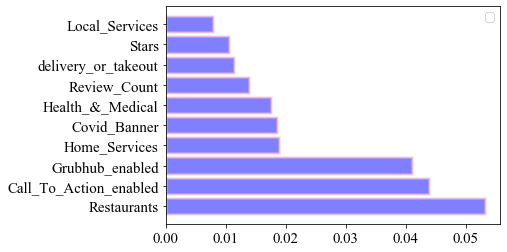
\includegraphics[width=0.7\linewidth]{signi_feature.png}
    \caption{The Top 10 most important features. For example, a weight of 0.05 means balanced-accuracy decreases by 5\% without the corresponding feature. }
    \label{fig:sig}  %
\end{figure*}


Based on Fig.~\ref{fig:sig}, COVID features like $\texttt{ Call\_To\_Action\_enabled, Grubhub\_enabled, Covid\_Banner} $, and $\texttt{delivery\_or\_takeout} $ are important in this classification task. It is also worth noting that Health\_\&\_Medical is an important feature. 



\section{Conclusions and Future Work}

\subsection{Conclusions}



In this paper, we build a comprehensive business dataset with rich features, collected from diverse information sources. Then we formulate the problem of predicting business survival and employed several machine learning methods to solve it. In this process, we develop an exhaustive training and evaluation pipeline combining techniques like SMOTE, cross validation and make use of multiple performance metrics. Results show that all models are significantly better at classifying open businesses than closed ones. Finally, we determine the 10 most important features that influence business survival. The presence of four COVID features suggests that a business' survival prospects are reliant on providing services that ensure customer health and safety. For eg, restaurants having Grubhub enabled. We hope that our work can help save the economy by informing and guiding business owners, investors and other people in power to make wise business decisions.  




\subsection{Future Work}
The Yelp dataset has a file called $\texttt{review.json}$ that contains reviews written by users for businesses. Users and Businesses are identified through $\texttt{user\_id}$ and $\texttt{business\_id}$ respectively. Natural Language Processing can be leveraged and this data can be used to perform sentiment analysis. This will give us a sense of what customers think about the business and this sentiment can be modelled as a feature to help us possibly obtain better classifiers. In addition to this we would also like to gather a larger dataset with more countries in order to build models that generalize better and aren't limited to specific countries. 







\pagebreak

\nocite{*}
\bibliographystyle{unsrt}
\bibliography{References.bib}



\newpage
\section{Appendix}

\subsection{Additional Machine Learning Models}
\subsubsection{Support Vector Machine Model}
Library:  $\texttt{sklearn.svm.LinearSVC()}$~\cite{SVM, svm_sklearn}

We use $\texttt{sklearn.svm.LinearSVC()}$ because $\texttt{sklearn.svm.SVC()}$ is not suitable for the large-scale dataset because of it time complexity. Here we choose $l_2$ norm to represent the distance between different features, and use squared hinge loss as our loss function.


\subsubsection{Naive Bayes}
Library:  $\texttt{mixed\_naive\_bayes.MixedNB}$~\cite{nblib}


\subsection{Additional Results}



\begin{table}[hbpt]
\begin{tabular}{p{4cm}|p{4cm}|p{3.5cm} |p{3.5cm} } 
 \hline

 Classifier & 10-Fold CV Balanced-Accuracy (\%) & Test Balanced-Accuracy (\%) & Test Vanilla Accuracy (\%)\\
 \hline
 Support Vector Machines  & 70.45 & 70.53  & 76.66\\
 Naive Bayes & 68.65 & 68.31  & 67.81 \\
 \hline

\end{tabular}
  \caption{Model Evaluation for  Support Vector Machines  and Naive Bayes} 
  \vspace{-2ex}
  \label{tab:table1}
\end{table}




\begin{table}[hbpt]
\centering
\begin{tabular}{ c|c|c|c|c|c|c }
 \hline
 ~& \multicolumn{3}{c|}{Class 0 (Closed Businesses)} & \multicolumn{3}{c}{Class 1 (Open Businesses)}  \\
 \hline
Model Type & Precision (\%) & Recall (\%) & F1  & Precision (\%) & Recall (\%) & F1 \\
 \hline
 Support Vector Machines & 40.67 & 60.88  & 48.76  & 90.18 & 80.17 & 84.88
 \\

  Naive Bayes & 32.19 & 69.10 & 43.92 & 90.73 & 67.52 & 77.42
 \\
 
 \hline

\end{tabular}
  \caption{Model Evaluation on Each Class for Support Vector Machines  and Naive Bayes} 
  \vspace{-2ex}
  \label{tab:table_class}
\end{table}




\end{document} 
































